\documentclass[border=0pt]{standalone}
\usepackage{amsmath,amssymb}
\usepackage{tikz}
\usetikzlibrary{arrows.meta,shadows,positioning,calc,decorations.pathreplacing}
\definecolor{acc}{HTML}{0D9488}
\definecolor{ink}{HTML}{1A1D21}
\definecolor{mut}{HTML}{646A72}
\definecolor{paper}{HTML}{F8F9FB}
\definecolor{bad}{HTML}{E05A47}
\tikzset{
  keep/.style={draw=acc!75!black, line width=1.3pt, fill=acc!22, rounded corners=5pt, minimum height=8.5mm, minimum width=12mm, font=\ttfamily\bfseries\Large, text=ink, drop shadow={opacity=0.25, shadow xshift=1.2pt, shadow yshift=-1.2pt}},
  cut/.style={draw=mut!70, line width=1pt, dashed, fill=white, rounded corners=5pt, minimum height=7.5mm, minimum width=10.5mm, font=\ttfamily\large, text=mut},
  edge/.style={-{Latex[length=2.6mm]}, line width=1.3pt, draw=acc!70!black},
  dead/.style={-{Latex[length=2.2mm]}, line width=0.9pt, draw=mut!60, dashed},
}
\newcommand{\cross}[1]{\draw[bad, line width=1.6pt] ($(#1.north east)+(0.06,0.06)$) -- ++(-0.28,-0.28) ($(#1.north east)+(-0.22,0.06)$) -- ++(0.28,-0.28);}
\begin{document}
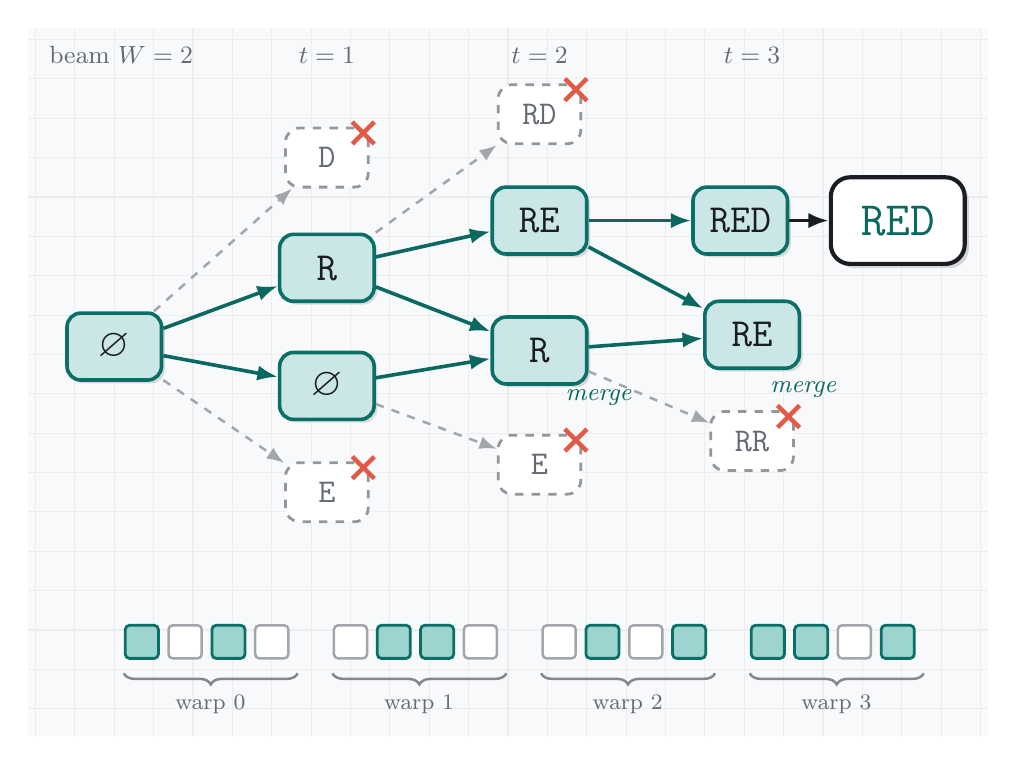
\begin{tikzpicture}
  \useasboundingbox (-1.1,-4.35) rectangle (11.1,4.65);
  \fill[paper] (-1.1,-4.35) rectangle (11.1,4.65);
  \draw[mut!12, step=0.5] (-1.1,-4.35) grid (11.1,4.65);

  \node[keep] (r0) at (0,0.6) {$\varnothing$};

  \node[keep] (a1) at (2.7,1.6) {R};
  \node[keep] (b1) at (2.7,0.1) {$\varnothing$};
  \node[cut]  (c1) at (2.7,3.0) {D};
  \node[cut]  (d1) at (2.7,-1.25) {E};

  \node[keep] (a2) at (5.4,2.2) {RE};
  \node[keep] (b2) at (5.4,0.55) {R};
  \node[cut]  (c2) at (5.4,3.55) {RD};
  \node[cut]  (d2) at (5.4,-0.9) {E};

  \node[keep] (a3) at (7.95,2.2) {RED};
  \node[keep] (b3) at (8.1,0.75) {RE};
  \node[cut]  (c3) at (8.1,-0.6) {RR};

  \foreach \f/\t in {r0/a1, r0/b1, a1/a2, a1/b2, b1/b2, a2/a3, a2/b3, b2/b3} \draw[edge] (\f) -- (\t);
  \foreach \f/\t in {r0/c1, r0/d1, a1/c2, b1/d2, b2/c3} \draw[dead] (\f) -- (\t);
  \foreach \n in {c1, d1, c2, d2, c3} {\cross{\n}}

  \node[font=\itshape\small, text=acc!70!black] at (6.15,-0.05) {merge};
  \node[font=\itshape\small, text=acc!70!black] at (8.75,0.05) {merge};

  \node[draw=ink, line width=1.5pt, fill=white, rounded corners=7pt, minimum height=11mm, minimum width=17mm, font=\ttfamily\bfseries\LARGE, text=acc!70!black, drop shadow={opacity=0.3, shadow xshift=1.5pt, shadow yshift=-1.5pt}] (out) at (9.95,2.2) {RED};
  \draw[edge, draw=ink] (a3) -- (out);

  \foreach \x/\t in {2.7/1, 5.4/2, 8.1/3} \node[font=\small, text=mut] at (\x,4.3) {$t=\t$};
  \node[font=\small, text=mut, anchor=west] at (-0.95,4.3) {beam $W=2$};

  \foreach \w in {0,...,3} {
    \foreach \i in {0,...,3} {
      \pgfmathsetmacro{\on}{mod(\w*4+\i*3,5) < 3 ? 1 : 0}
      \pgfmathsetmacro{\xx}{0.35 + \w*2.65 + \i*0.55}
      \ifdim\on pt>0.5pt
        \node[draw=acc!75!black, fill=acc!40, line width=1pt, rounded corners=1.5pt, minimum size=4.2mm, inner sep=0] at (\xx,-3.15) {};
      \else
        \node[draw=mut!60, fill=white, line width=0.9pt, rounded corners=1.5pt, minimum size=4.2mm, inner sep=0] at (\xx,-3.15) {};
      \fi
    }
    \draw[mut!80, line width=0.9pt, decoration={brace, mirror, amplitude=4pt}, decorate] (0.12+\w*2.65,-3.55) -- (2.33+\w*2.65,-3.55);
    \node[font=\footnotesize, text=mut] at (1.22+\w*2.65,-3.95) {warp \w};
  }
\end{tikzpicture}
\end{document}
